\documentclass[xcolor=dvipsnames, 12pt]{beamer}
\useoutertheme{infolines} 
%\definecolor{grayish}{RGB}{147,162,153}
\usecolortheme[named=gray]{structure} 
\usetheme[height=7mm]{Rochester}

\usepackage{graphicx}

\usepackage{AMMALanguages}
\usepackage{hyperref}
\usepackage{tikz}
\usetikzlibrary{positioning}
\usetikzlibrary{arrows,shapes}

%\setbeameroption{show notes}
%\setbeameroption{show only notes}
\setbeamertemplate{note page}[plain]

\usepackage[utf8]{inputenc}
\usepackage[T1]{fontenc}

\usepackage{listings}

\newcommand\blfootnote[1]{%
  \begingroup
  \renewcommand\thefootnote{}\footnote{#1}%
  \addtocounter{footnote}{-1}%
  \endgroup
}

\AtBeginSection{\frame{\sectionpage}}

\title[Verifying ATL]{Fully Verifying Transformation Contracts for Declarative ATL}
%\title{Full Verification of Model Transformation Contracts for Declarative ATL}
\author[Oakes, Troya, Lucio, Wimmer]{\textbf{Bentley James Oakes}, Javier Troya, Levi L\'{u}cio, Manuel Wimmer}
%\subtitle{}
%\logo{}
\institute[]{McGill University, Canada\\Vienna University of Technology, Austria}
%\date{}
%\subject{}
%\setbeamercovered{transparent}
%\setbeamertemplate{navigation symbols}{}

% logo of my university
\titlegraphic{\vspace{-0.5cm}\includegraphics[width=3cm]{figures/mcgill}\hspace*{4.75cm}~%
   \includegraphics[width=4cm]{figures/big}
}

\begin{document}
\maketitle

%\section{Intro}

\begin{frame}{Motivation}
\begin{itemize}[<+->]
\item Model transformations are at the heart of model-based engineering
\item Atlas Transformation Language (ATL) is increasingly used in industry
\begin{itemize}
\item Example: Generating code to/from models
\end{itemize}

\item Want to verify correctness for ATL transformation specifications
\begin{itemize}[<+->]
\item Verify visual contracts
\item Input independence - verification for all input models
\item Examine combinations of transformation rules
\end{itemize}
\end{itemize}
\end{frame}

\begin{frame}{Overview}

\begin{itemize}[<+->]
\item Translating ATL transformation into DSLTrans language
\item Verify visual contracts on DSLTrans
\end{itemize}
\begin{center}
\includegraphics[width=\textwidth]{figures/overview}
\end{center}
\begin{itemize}[<+->]
\item Performed through a higher-order transformation
\begin{itemize}
\item Specified in ATL
\end{itemize}
\end{itemize}
\end{frame}


%\section{Families-To-Persons Transformation}

\begin{frame}{Transformation Metamodels}

\begin{center}
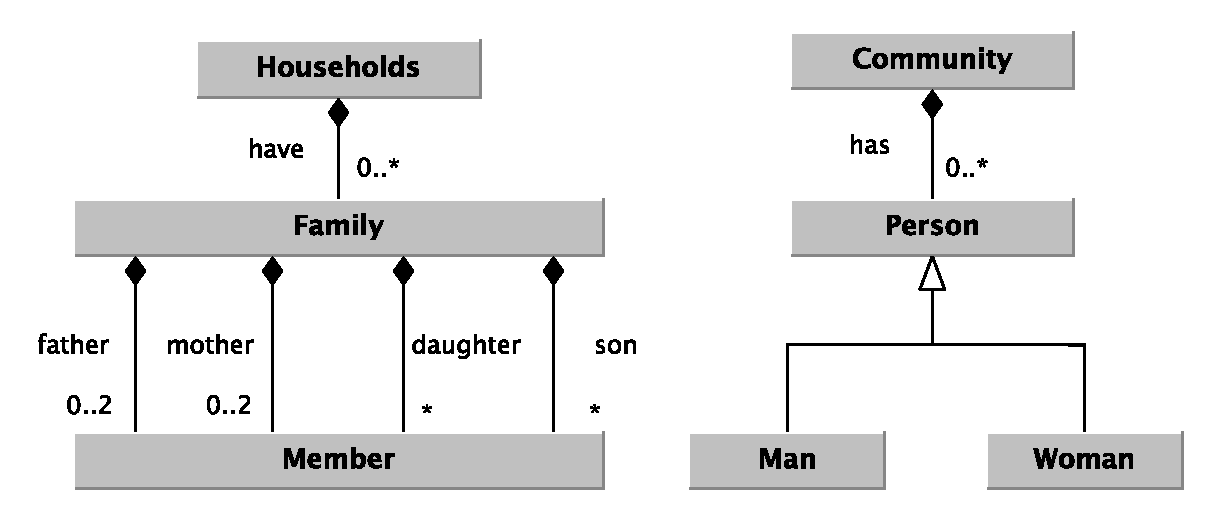
\includegraphics[width=0.8\textwidth]{figures/Metamodels_F2P}
\end{center}
\begin{itemize}[<+->]
\item Transform \textit{Members} to \textit{Men} and \textit{Women}
\item NB: Metamodels are not representative of today's society!
\end{itemize}
\end{frame}

\begin{frame}{ATL Transformation}
\begin{center}
\includegraphics[width=0.8\textwidth]{figures/ATL_code_first}
\end{center}
\end{frame}

\begin{frame}{ATL Transformation}
\begin{center}
\includegraphics[width=0.8\textwidth]{figures/ATL_code}
\end{center}
\pause
\begin{itemize}
\item Implicit resolution mechanism of ATL
\item Through collect operation
\end{itemize}
\end{frame}

\begin{frame}{DSLTrans Transformation}

\begin{itemize}[<+->]
\item Visual language for model transformations
\item Graph-based, contains rules arranged in layers

\end{itemize}
\pause
\begin{itemize}[<+->]
\item Out-place so no rewriting performed, only production
\begin{itemize}
\item Suited for `translation' transformations
\end{itemize}
\item All DSLTrans computations are terminating and confluent
\item Unbounded loops during execution are not allowed
\end{itemize}
\end{frame}

\begin{frame}{DSLTrans}
\begin{center}
\includegraphics[width=\textwidth]{figures/Rules}
\end{center}

\begin{itemize}
\item Rules arranged in layers
\item Match graph on top of rules
\item Apply graph on bottom
\begin{itemize}
\item Produced when match graph is found
\end{itemize}
\end{itemize}
\end{frame}

\begin{frame}{Mapping - Part One}
\begin{itemize}
\item Higher-order transformation written in ATL
\item Creates a DSLTrans transformation from declarative ATL
\begin{itemize}
\item Informal testing: less than 20 seconds
\end{itemize}
\item Available on our website: \url{http://msdl.cs.mcgill.ca/people/levi/files/MODELS2015}
\end{itemize}
\end{frame}


\begin{frame}{Mapping - Part Two}
\begin{center}
\includegraphics[width=\textwidth]{figures/features}
\end{center}

\begin{itemize}
\item Covers declarative ATL
\item Transformation can be rewritten to avoid missing features
\end{itemize}
\end{frame}

\begin{frame}{Mapping - Part Three}
\begin{itemize}[<+->]
\item Two steps for higher-order transformation
\item First, each from/to part of an ATL rule is transformed into match/apply graphs in DSLTrans
\item Attributes will also be set in these rules
\item Second, DSLTrans rules are produced for any bindings in the ATL rule
\end{itemize}


\end{frame}

\begin{frame}{Mapping - Part Four}
\begin{center}
\includegraphics[width=0.9\textwidth]{figures/ATL_collect}
\end{center}
\begin{center}
\includegraphics[width=\textwidth]{figures/Rules}
\end{center}
\end{frame}

%\begin{frame}{SyVOLT Tool}
%\begin{itemize}
%\item Eclipse plugin frontend to create transformations and contracts in visual editor
%\item Python backend to prove contracts 
%\item SyVOLT: Full Model Transformation Verification Using Contracts\\Levi Lucio, Bentley James Oakes, Claudio Gomes, Gehan M. K. Selim, Juergen Dingel, James R. Cordy and Hans Vangheluwe. 
%\end{itemize}
%\end{frame}




\begin{frame}{Contracts}
\begin{center}
\includegraphics[width=0.50\textwidth]{figures/fourMembersProp}
\end{center}
\pause
\begin{itemize}[<+->]
\item If blue graph is in input model, then red graph is in output model
\item Objective: Prove for all input models/transformation executions
\item \textit{A family with a father, mother, son, daughter
should always produce two males and two females in the
target community}
\end{itemize}
\end{frame}


\begin{frame}{Contracts}
\begin{center}
\includegraphics[width=0.48\textwidth]{figures/motherFatherProp}
\end{center}
\pause
\begin{itemize}[<+->]
\item Reasoning about attributes of elements
\item \textit{Is the full name of the produced Person correctly created from the last name of the Family and the first name of the Member?}
\end{itemize}
\end{frame}

\begin{frame}{Contracts}
\begin{center}
\includegraphics[width=0.7\textwidth]{figures/daughterMotherProp}
\end{center}
\begin{itemize}[<+->]
\item A contract that will not hold
\item \textit{A family with a mother and a daughter will always produce a community with a man}
\end{itemize}
\end{frame}



\begin{frame}{Contract Proving - Part One}
\begin{itemize}[<+->]
\item SyVOLT contract proving tool
\item All possible executions of the transformation are symbolically constructed
\begin{itemize}[<+->]
\item Built as sets of rules called path conditions
\begin{itemize}
\item No rules execute, only rule 1 executes, rule 1 and rule 2 both execute
\item Rule dependencies/combinations resolved
\end{itemize}
\item Final set of path conditions represents all possible transformation executions
\end{itemize}
\item A contract holds for a transformation if it holds for all generated path conditions
\end{itemize}
\blfootnote{L. Lúcio, B. Oakes, and H. Vangheluwe. A technique for symbolically verifying properties of graph-based model transformations. Tech. Report SOCS-TR-2014.1, McGill U, 2014.}
\blfootnote{Levi Lucio et al. SyVOLT: Full Model Transformation Verification Using Contracts}
\end{frame}

%\section{Mapping ATL to DSLTrans}

\begin{frame}{Contract Proving - Part Two}
\begin{center}
\includegraphics[width=0.7\textwidth]{figures/daughterMotherProp}
\end{center}
\begin{itemize}[<+->]
\item \textit{A family with a mother and a daughter will always produce a community with a man}
\item Fails on path condition: 'HEmpty\_HRoot\_HMotherRule\_HDaughterRule'
\end{itemize}
\end{frame}

%\section{Generating Path Conditions}



%\section{Results}

\begin{frame}{Experiments Conducted}
\begin{itemize}
\item Applicability of the Technique
\item Time and Memory Characteristics
\item Reducing Contract Proving Time
\item Higher-Order Transformation
\end{itemize}
\end{frame}

\begin{frame}{Applicability of the Technique - Part One}
\begin{itemize}[<+->]
\item Applied to multiple transformations from ATL zoo
\begin{itemize}[<+->]
\item Ranging in size from 5-15 ATL rules
\end{itemize}
\begin{itemize}[<+->]
\item Example below:
\item Ecore Copier transformation - 11 ATL rules, 24 DSLTrans rules
\item Copies Ecore elements in input model to output model
\end{itemize}
\end{itemize}
\pause
\begin{center}
\includegraphics[width=0.45\textwidth]{figures/Ecore_copier_prop1}
\end{center}
\end{frame}

\begin{frame}{Applicability of the Technique - Part Two}
\begin{itemize}
\item Technique works with attributes on elements
\begin{itemize}
\item Proving names of people correctly created
\end{itemize}
\end{itemize}
\pause
\begin{center}
\includegraphics[width=0.45\textwidth]{figures/motherFatherProp}
\end{center}
\end{frame}

\begin{frame}{Applicability of the Technique - Part Three}
\begin{center}
\includegraphics[width=\textwidth]{figures/communityPersonProp}
\end{center}
\pause
\small
\vspace{-0.8cm}
\begin{itemize}
\item \textit{`If a Community is connected to a Person element, that Community is connected
to one and only one Person element'}
\item Selim, Gehan. Formal Verification of Graph-Based Model Transformations. PhD Diss. Queen’s University, 2015.
\end{itemize}
\end{frame}

\begin{frame}{Time and Memory Characteristics}
\begin{center}
\includegraphics[width=\textwidth]{figures/top_table}
\end{center}
\pause
\begin{itemize}
\item Feasible
\begin{itemize}[<+->]
\item Time - Ranging from 0.5 seconds to 48 minutes (on laptop)
\item Memory - 43 to 7800 MB RAM/disk usage
\item (Both measures have been improved in newer tool versions)
\end{itemize}
\end{itemize}
\end{frame}

\begin{frame}{Reducing Contract Proving Time}
\begin{center}
\includegraphics[width=\textwidth]{figures/middle_table_2}
\end{center}
\begin{itemize}[<+->]
\item Examined ATL transformation which is transformed into 63 DSLTrans rules
\item To make feasible, need to slice transformation based on contract
\item Procedure:
\begin{itemize}[<+->]
\item Find rules that create contract elements
\item Recursively create rule dependency tree
\end{itemize}
\item Manually performed - slicing has since been automated
\end{itemize}
\end{frame}

\begin{frame}{Higher-Order Transformation}
\begin{itemize}
\item Question: Is a transformation produced by a HOT equivalent to a hand-built one?\blfootnote{G. M. Selim, L. Lúcio, J. R. Cordy, J. Dingel, and B. J. Oakes. Specification and verification of graph-based model transformation properties.
In Graph Transformation, pages 113–129. Springer, 2014.}
\end{itemize}
\pause
\begin{center}
\includegraphics[width=\textwidth]{figures/bottom_table_2}
\end{center}
\pause
\begin{itemize}
\item Note that number of rules/transformation shape not optimized
\item But HOT produces roughly equivalent result 
\end{itemize}
\end{frame}

%\section{Conclusion and Thanks}

\begin{frame}{Conclusion}
\begin{itemize}[<+->]
\item Developed higher-order transformation to transform ATL into DSLTrans
\item Can verify visual contracts on DSLTrans transformations in feasible time
\item Contracts verified on all transformation executions
\item Future work
\begin{itemize}
\item Integrate HOT into SyVOLT tool
\item Investigate contract-based transformation development
\end{itemize}
\end{itemize}
\pause
\begin{itemize}
\item Thank you for your time!
\end{itemize}
\begin{center}
\textbf{Fully Verifying Transformation Contracts for Declarative ATL}\\
\textbf{Bentley James Oake}s, Javier Troya, Levi L\'{u}cio, and Manuel Wimmer\\
McGill University, Canada\\Vienna University of Technology, Austria\\
\url{http://msdl.cs.mcgill.ca/people/levi/files/MODELS2015}

\end{center}
\end{frame}

\begin{frame}{Multiplicity Contract}
\begin{center}
\includegraphics[width=\textwidth]{figures/multi}
\end{center}
``Multiplicity Invariants ensure that the transformation does not produce an output that violates the multiplicities in the Kiltera metamodel''
\end{frame}

\begin{frame}{Syntactic Invariant}
\begin{center}
\includegraphics[width=\textwidth]{figures/syn}
\end{center}
``Syntactic Invariants ensure that the generated Kiltera output model is well-formed with respect to Kiltera's syntax.''
\end{frame}

\begin{frame}{Pattern Contracts}
\begin{center}
\includegraphics[width=\textwidth]{figures/patt}
\end{center}
``Pattern contracts require that if a certain pattern of elements exists in the input
model, then a corresponding pattern of elements exists in the output model''
\end{frame}

\end{document}
